\documentclass[x11names]{book}

  \usepackage[total={8cm,21cm},top=2cm, left=2cm]{geometry}
\usepackage{amsthm,amsmath,amssymb,amsfonts,xcolor}
\usepackage[latin1]{inputenc}
\definecolor{azulF}{rgb}{.0,.0,.3} % Azul
\definecolor{rojoF}{RGB}{212,0,0} % Rojo
\newcommand{\Z}{\mathbb{Z}} % \Z

\usepackage{tcolorbox, empheq}%
\tcbuselibrary{skins,breakable,listings,theorems}
\tcbset{opteqA/.style={%
tcboxraise base,
nobeforeafter,
extrude by=-2mm,
colback=red!50!black!20,
colframe=red!50!black!20}}


\begin{document}

\tcbset{CajaconCapas/.style={%
colback=yellow!2, % Color de fondo
enlarge top by=1cm, % Espacio arriba (por la imagen)
enhanced, % Habilitar c�digo TikZ
breakable, % habilitado el quiebre de caja
boxrule=0pt, % sin borde (0pt)
top=7mm, % espacio vertical del borde al texto = 7mm
drop fuzzy shadow, % sombra
overlay unbroken = {
% Barra vertical
% xshift = corrimiento horizontal
% yshift = corrimiento vertical
\draw[color=red!80!yellow,line width =3pt]
([xshift=2pt] frame.north west)--([xshift=2pt] frame.south west);
% Barra horizontal
\draw[color=red!80!yellow,line width =1pt]
( frame.north west)--(frame.north east);
% Caja de imagen
\node[rectangle] at ([xshift=1cm,yshift=0.45cm]frame.north west)
{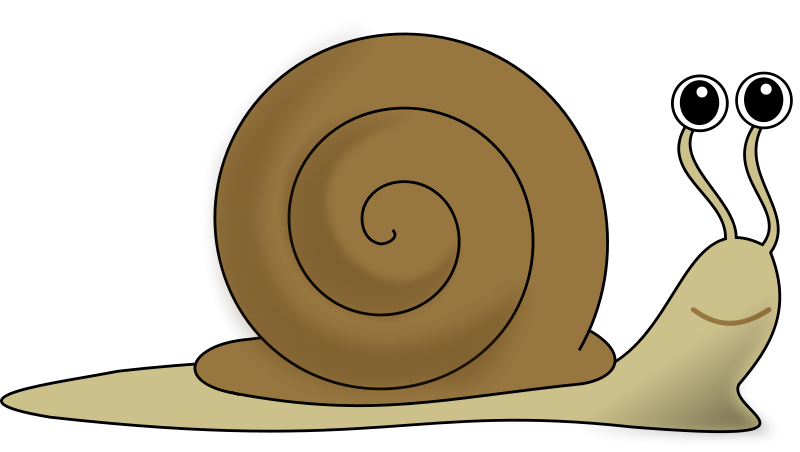
\includegraphics[scale=0.06]{images/caracol}};
% Caja de descripci�n
% minimum width = tama�o m�nimo del rect�ngulo
\node[rectangle, draw=DeepSkyBlue1, fill=DeepSkyBlue1,
font=\LARGE\bfseries, text=white, rounded corners=8pt,minimum width =3cm
,
inner sep=1mm,anchor=north west] at
([xshift=4cm,yshift=0.3cm]frame.north west){ Gu�a};
},
overlay first = {% capa superior
% Barra vertical
\draw[color=red!80!yellow,line width =3pt]
([xshift=2pt] frame.north west)--([xshift=2pt] frame.south west);
% Barra horizontal
\draw[color=red!80!yellow,line width =1pt]
( frame.north west)--(frame.north east);
% Caja de imagen
\node[rectangle] at ([xshift=1cm,yshift=0.45cm]frame.north west)
{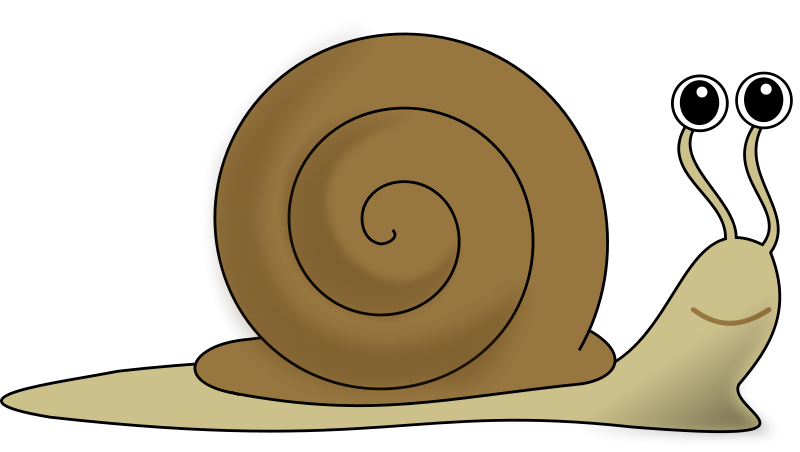
\includegraphics[scale=0.06]{images/caracol}};
% Caja de descripci�n
% minimum width = tama�o m�nimo del rect�ngulo
\node[rectangle, draw=DeepSkyBlue1, fill=DeepSkyBlue1,
font=\LARGE\bfseries, text=white, rounded corners=8pt,minimum width =3cm
,
inner sep=1mm,anchor=north west] at
([xshift=4cm,yshift=0.3cm]frame.north west){ Gu�a};
}, %First
% Lo que permanece ante cambio de p�ginas
overlay middle = { % Barra vertical
\draw[color=red!80!yellow,line width =3pt]
([xshift=2pt] frame.north west)--([xshift=2pt] frame.south west);
},
% Permanece la barra vertical
overlay last={\draw[color=red!50!black!50,line width =3pt]
([xshift=3pt] frame.north west)--([xshift=2pt] frame.south west);
}
}}



% Usando el entorno
\begin{tcolorbox}[CajaconCapas]
\begin{enumerate}
\item Abra un nuevo archivo en GeoGebra.\\
\item Oculte los ejes, para esto elija el men� ...
\item Elija la herramienta Pol�gono y construya ...
\item Utilice la herramienta Punto Medio o Centro ...
\end{enumerate}
\end{tcolorbox}


\end{document}